\documentclass[a4paper]{jpconf}
\usepackage{graphicx}
\begin{document}
\title{DBSSql}

\author{Anzar Afaq, Vijay Sekhri, Yuyi Guo, Lee Lueking}
\address{Fermilab, Batavia, Illinois, USA}

\author{Valentin Kuznetsov}
%\author{Valentin Kuznetsov, Daniel Riley}
\address{Cornell University, Ithaca, NY 14853, USA}

\begin{abstract}
The CMS experiment has implemented a flexible and 
powerful approach enabling users to find data within 
the CMS physics data catalog. The Dataset Bookkeeping 
Service (DBS) comprises a database and the services 
used to store and access metadata related to its physics 
data. In addition to the existing WEB based and programmatic 
API, a generalized query system has been designed and built. 
This query system has a query language that hides the 
complexity of the underlying database structure. This provides 
a way of querying the system that is straightforward for 
CMS data managers and physicists. The DBS Query Language 
uses the ANTLR tool to build the input query parser and tokenizer, 
then a query builder using a graph representation of the 
DBS schema constructs the actual SQL sent to underlying database. 
We will describe the design of the query system and provide 
details of the language components. We will also provide an 
overview of how this component fits into the overall data 
discovery system, as well as providing access to information 
about Data Quality and Luminosity.
\end{abstract}

\section{Introduction}
Introducetion text

\section{ITEMS TO COVER}
\begin{enumerate}
\item Need for a flexible QL, instead of static web pages
\item QL as Data search tool, and not a data mining tool (as of yet)
\item Some (not a whole lot !!!) implementation details.
\item Integration with DD and CLI
\item Future plans, DAS and beyond and also looking at Data Mining..
\end{enumerate}


\section{DBSql Architecture}
DBS QL architecture is shown on Pic. \ref{DBS_QL}.
% Here is example of how insert picture in LaTeX.
\begin{figure}[htb]
\centering
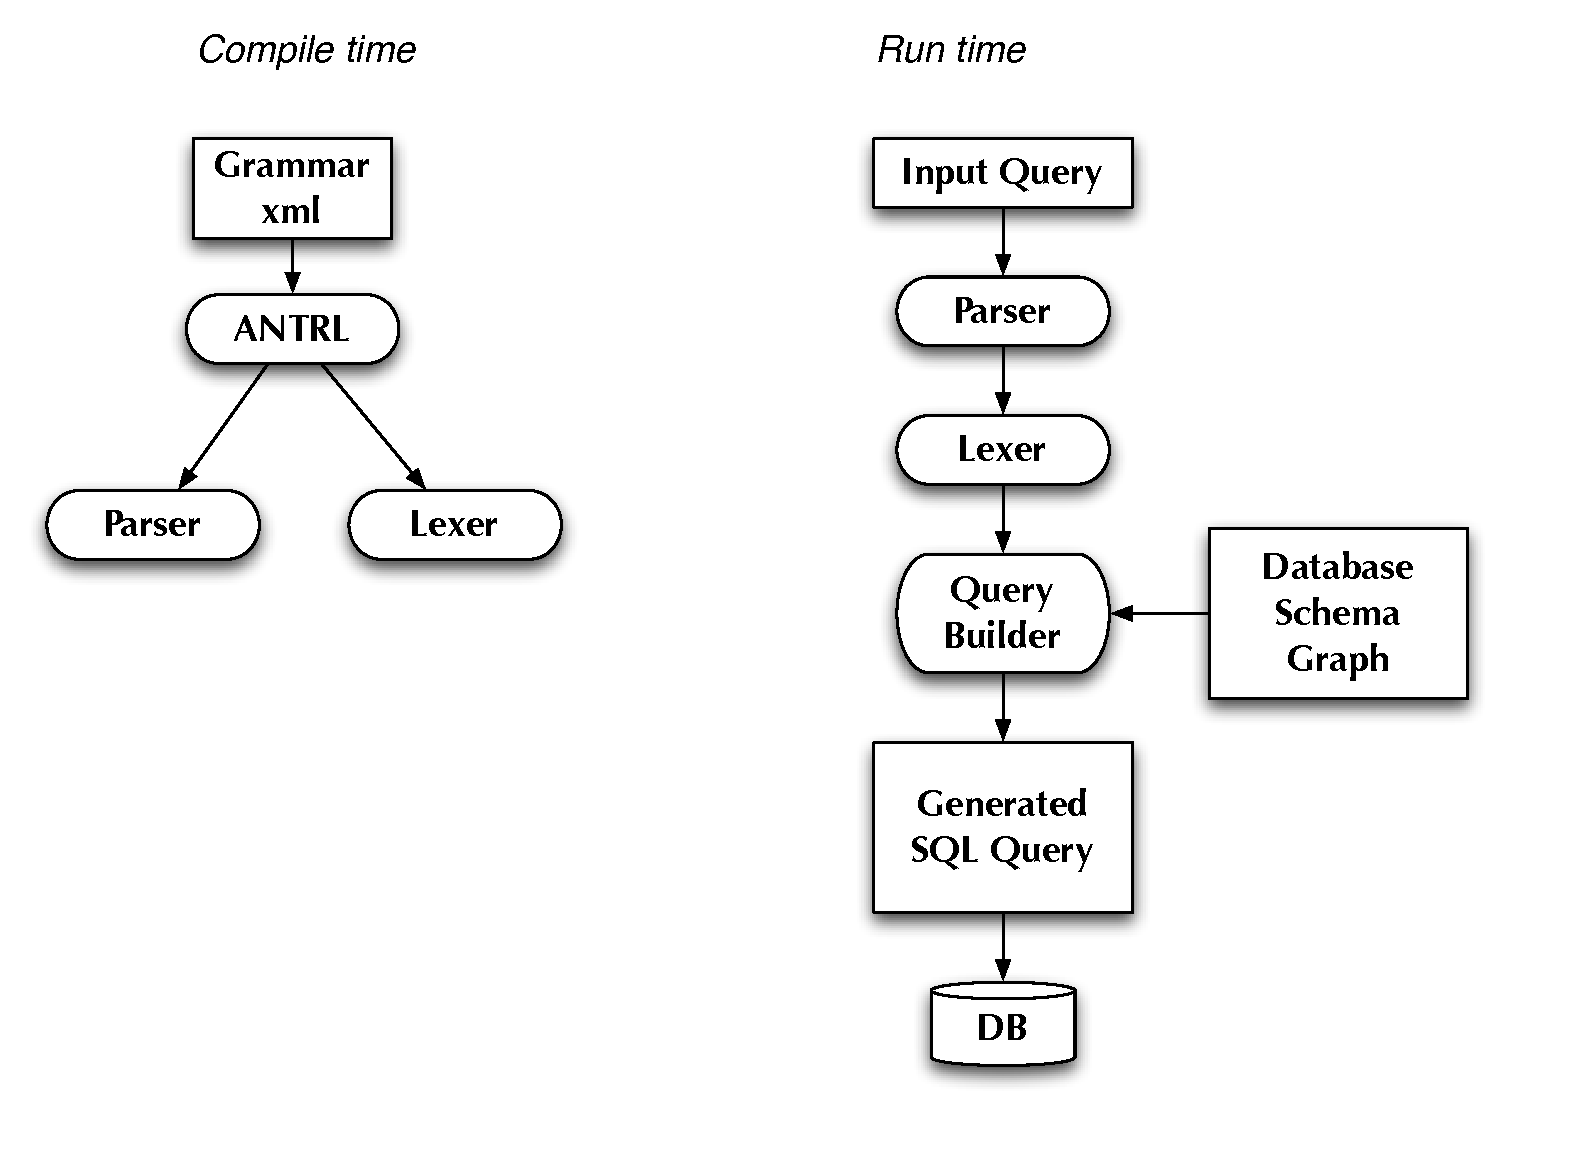
\includegraphics[width=100mm]{DBS_QL_architecture.pdf}
\caption{DBS QL architecture.}
\label{DBS_QL}
\end{figure}

The user input is interpreted by a lexer and parser, 
then a Query Builder generates the SQL query that can be executed on 
the database. The ANTLR \cite{ANTLR} parser/lexer tool 
usesa grammar file which defines the syntax and semantics for 
DBSql to generate the parsing/lexing code for compile time. 
The Query Builder package uses this parser and lexer to interpret 
the user input query. If the query does not honor the semantics of the 
grammar, then the parser or lexer will raise an exception. 
The Query Builder generates the final SQL query that is executed
directly on the DBS underlying MySql or Oracle database. 
The entire database schema is representedas a weighted
directed graph with nodes representing tables, and edges 
representing relationships between tables. The Query Builder
then uses the Dijkstra’s shortest path algorithm to determine a 
path from one table to another and resolve multi-path ambiguities.
The chosen path is used to construct the final SQLquery. 


For example the Fig. \ref{ShortestPath} shows database tables 
T1 through T4  where edges between the tables represents the 
relationships between the tables. The user can select elements
from table T1 and T4 without specifying intermediate tables T2 
and T3 and the join conditions. The Query Builder determines
the shortest path 
T1$\rightarrow$T2$\rightarrow$T3$\rightarrow$T4 
to add the intermediate tables 
and join conditions in the final SQLquery. 

\begin{figure}[htb]
\centering
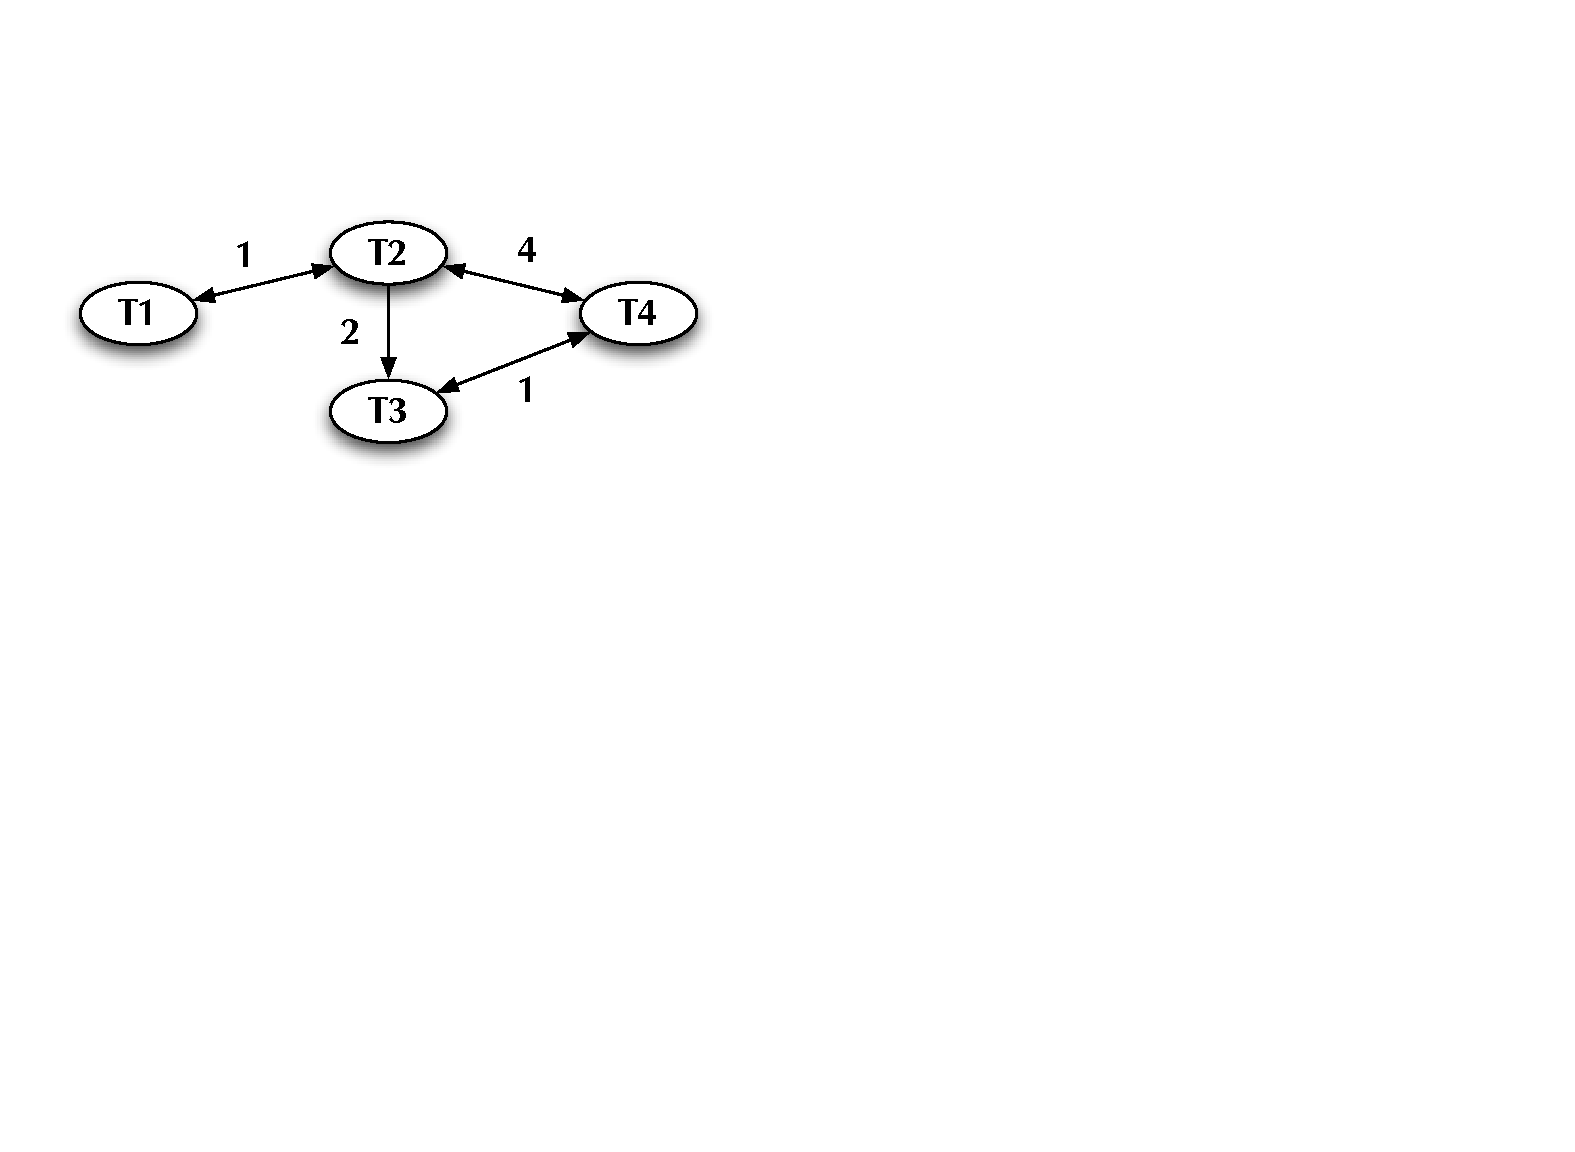
\includegraphics[width=150mm]{DBSSql_shortestpath.pdf}
\caption{
Shortest path from table T1 to T4 is 
T1 $\rightarrow$ T2 $\rightarrow$ T3 $\rightarrow$ T4  (Total weight 4) 
Shortest path from table T4 to T1 is 
T4 $\rightarrow$ T2 $\rightarrow$ T1 (Total weight 5) 
}
\label{ShortestPath}
\end{figure}

\section{DBS QL Grammar}


The figure represents a simplified view of the grammar
that defines the semantics of the DBSql. Entities are
like logical tables, and each entity has a set of additional 
attributes (table’scolumns). The grammar allows any 
combination of attribute and entity, however not 
every attribute is appropriate for each entity.
An incorrect combination will be detected by the Query Builder. 
Additional functions to count and sum items returned, e.g.
number of files and file sizes respectively,
make the language a powerful tool for generating
summaries. 

\begin{figure}[htb]
\centering
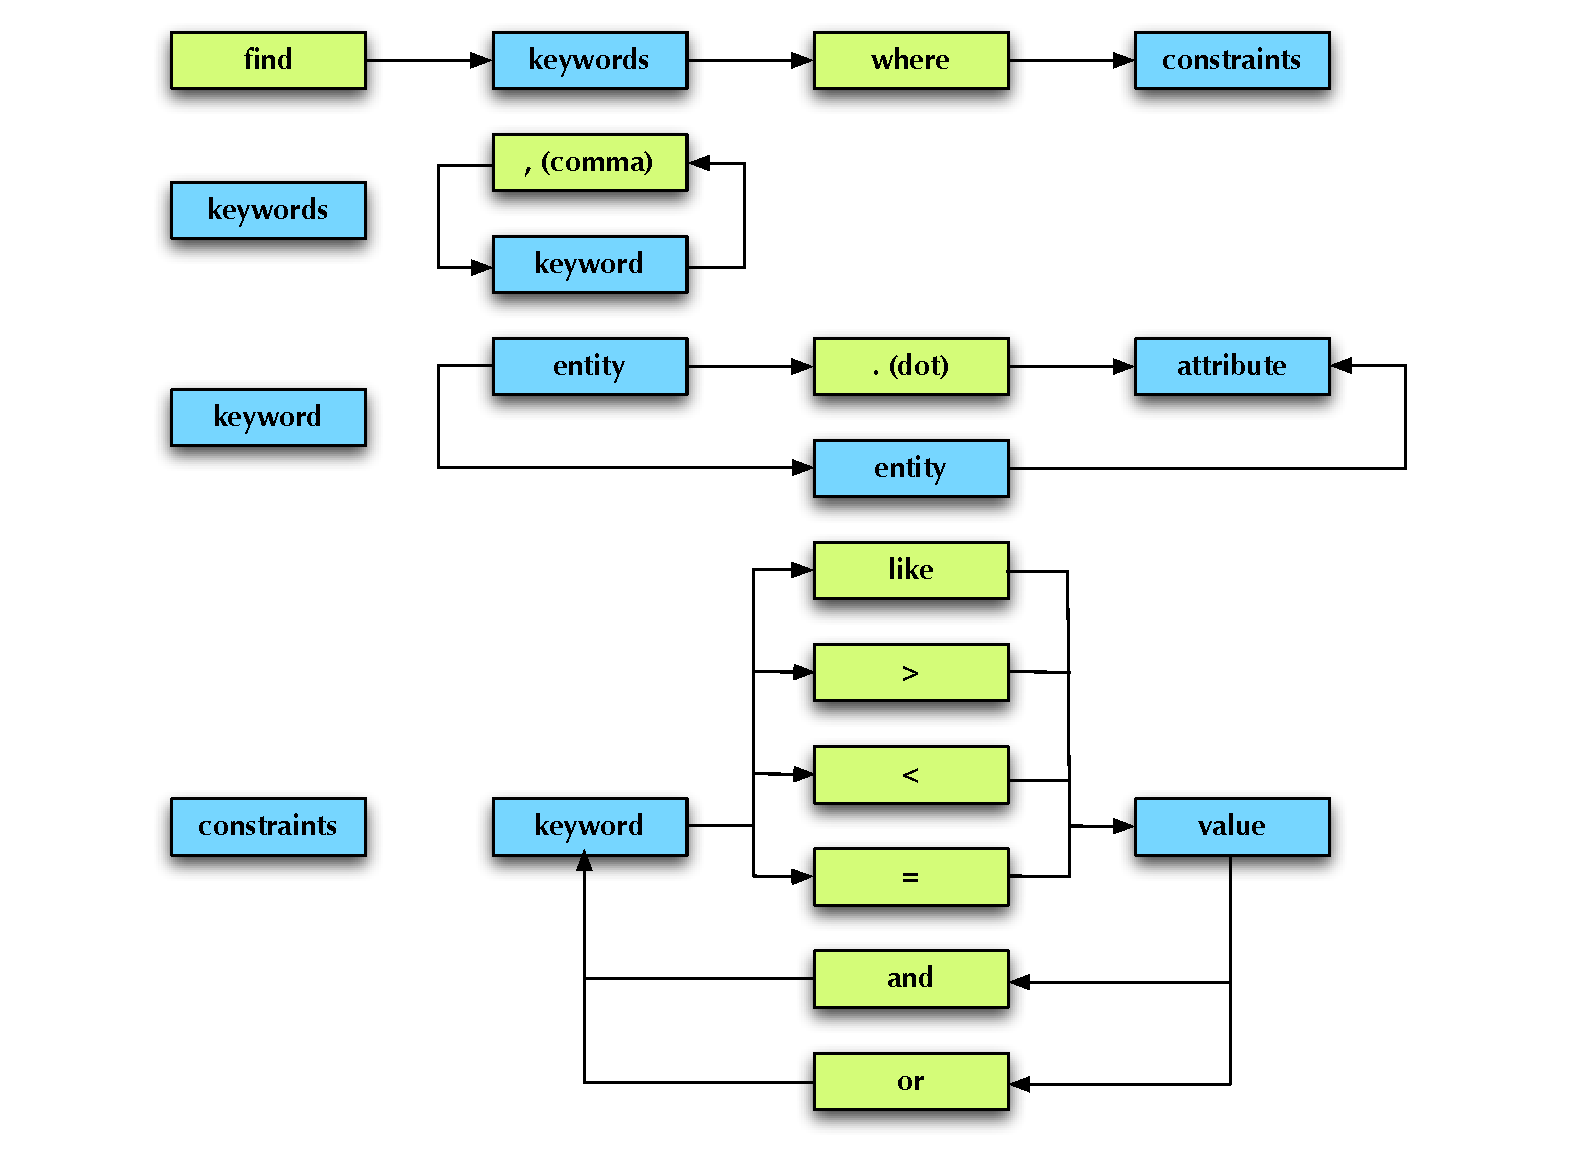
\includegraphics[width=150mm]{DBSSql_grammar.pdf}
\caption{
DBS QL grammar.
}
\label{ShortestPath}
\end{figure}

The keywords(entity or entity.attribute) used in DBSql 
are natural within the CMS community. Each keyword maps 
in to a particular 
table or table.column in the underlying database. 
The mapping of these keywords to the table.column are
maintained in a static file that models the graph
representation of the entire schema.

\section{Acknowledgements}

This work was supported by National Science Foundation.

\section*{References}
\begin{thebibliography}{9}
\bibitem{DBS} A. Afaq, et. al. ``The CMS Dataset Bookkeeping Service'', CHEP 2007 
\bibitem{ANTLR} http://www.antlr.org

\end{thebibliography}

\end{document}


